\section{Efficiency of Instrumented Code}
\label{sec:Efficiency}

The goal of PEBIL is to provide a toolkit that enables the construction of
instrumentation tools that produce efficient instrumented executables.
Specifically PEBIL is designed to provide efficiency when there are a large
number of instrumentation points because it is these cases where instrumentation
has the largest overhead on application performance. Several techniques are
employed to produce efficient instrumented code. One such technique is the use
of fast constructs to get control to the instrumentation code, which requires
the application code to be relocated and transformed. PEBIL also allows the use
of lightweight instrumentation snippets that can be used in place of
instrumentation functions for simple instrumentation tasks.

\subsection{Code Relocation and Transformation}
\label{Subsection:Relocation}
The use of relocation at the function level in PEBIL stems from the fact that
instrumentation is being performed statically on a platform that uses a
variable-length instruction set. The presence of variable-length length
instructions means that it may not always be possible to instrument an arbitrary
point using traditional techniques due to the lack of space at the
instrumentation point for a jump instruction large enough to reach the
instrumentation code. A common strategy used by static instrumentation toolkits
on platforms with fixed-length instruction sets is to replace a single
instruction at the instrumentation point with a branch instruction that will
transfer control to the instrumentation code. This is fairly straightforward
because, by the definition of a fixed-length instruction set, the instruction
being replaced and the replacing jump instruction have the same length. In x86
platforms, a jump instruction that uses a 32-bit offset requires 5 bytes.
However, for some instrumentation points of interest there may not be enough
space to hold a 5 byte jump instruction because the instrumentation point itself
(which might be an instruction or a basic block) is smaller than 5 bytes. 

Figure \ref{fig:InstructionSizes} shows a breakdown of the sizes of instructions
for a set of the SPEC CPU2000 Integer benchmarks. This figure shows that for
these benchmarks, between 52\% and 74\% of instructions are smaller than 5
bytes. In fact an average of 64\% of instructions are smaller, which indicates
that the the generic technique of replacing an instruction with a branch to
instrumentation code cannot provide instrumentation to large portions of the application
code.

\begin{figure}[ht]
\centering
\label{fig:InstructionSizes}
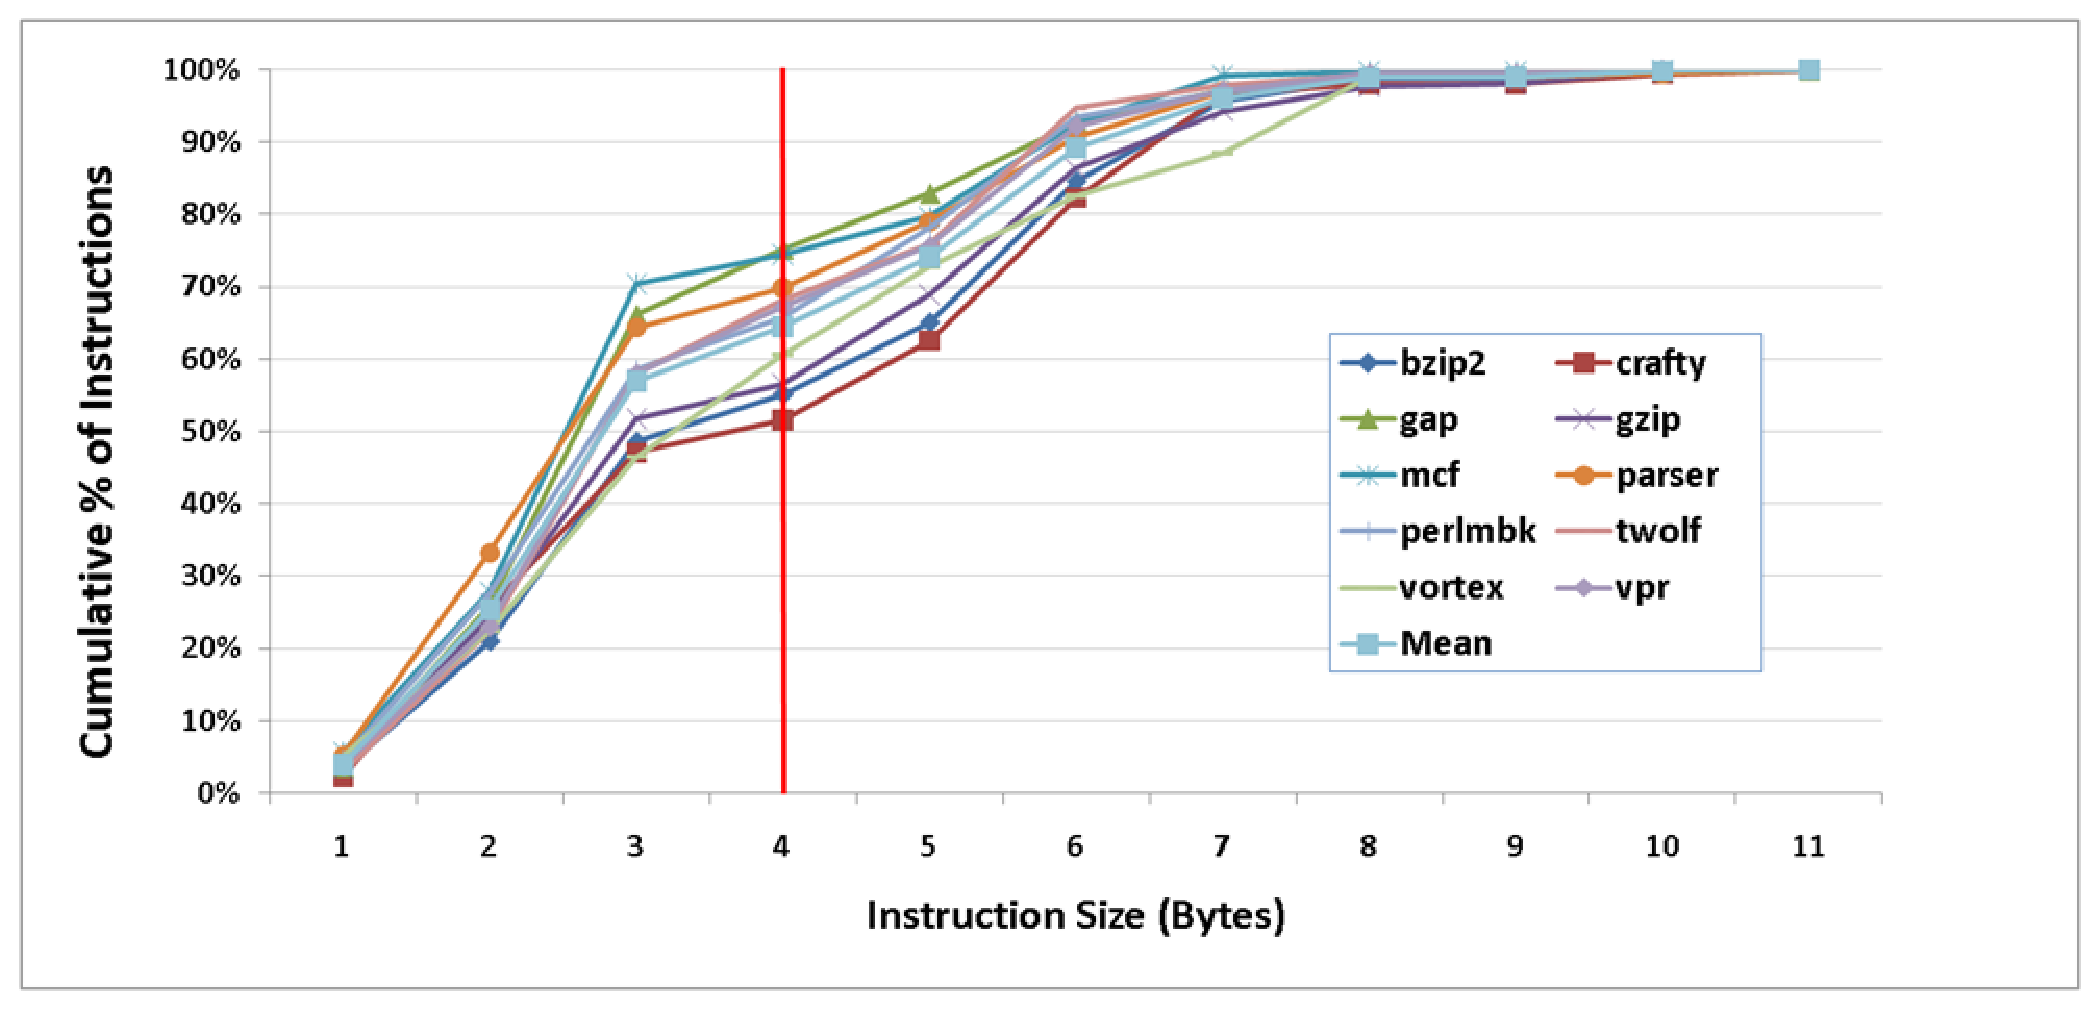
\includegraphics[scale=0.4]{instsize.eps}
\caption{Instruction sizes for a set of benchmarks presented on a cumulative basis.}
\end{figure}

This leaves two options for techniques that can be used to transfer control to
the instrumentation code. Either a technique entirely distinct from the idea of
using a single unconditional branch to execute the control transfer must be used
or somehow the application code must be altered in such a way that it can
accommodate a single large control instruction that is larger than the original
amount of space available at the instrumentation point. One alternative
technique for transferring control flow to an arbitrary point in the
instrumentation code could be to use a series of branches, where the instruction
at the instrumentation point is a small branch that transfers control to a
larger intermediate branch which in turn delivers control to the instrumentation
code. This method is unsatisfactory because the smallest traditional branch
instruction available on the x86 platform is 2 bytes in length, yet there are
instrumentation points with only a single byte available to them. Refer again to
Figure \ref{fig:InstructionSizes}, which shows that an average of 4\% of
instructions use only a single byte. Besides, this technique requires additional
space to be available in close proximity to the instrumentation points since
these smaller 2-byte branches are also short reaching, which is unlikely to be
available since function are often packed tightly within the application text.

Another option is the method proposed by the BIRD project \cite{nanda2006bird},
which is to use a single-byte \begin{it}INT3\end{it} instruction when a larger
traditional branch does not fit at the instrumentation point. This instruction
is functionally perfect for static instrumentation because it consumes only a
single byte and allows us to transfer control to an arbitrary location by using
the exception handling facilities provided by the system. A cursory study was
performed on this scheme from an efficiency standpoint to determine whether it
was worth further investigation. On a small benchmark set, a simple
implementation of using \begin{it}INT3\end{it} only when 5 byte branches do not
fit at the instrumentation point introduces slowdown of at least 100X for even
the simple task of counting the number of executions of each basic block in the
code. As one might expect, this mechanism is unsuitable for efficient
instrumentation because the heavyweight system call conventions are being
invoked on a fairly regular basis to transfer control between the application
and the instrumentation code.

PEBIL uses relocation and reorganization of the code at the function level which
provides is enough space at each instrumentation point to accommodate a 5 byte
jump. Specifically, the steps used by PEBIL to relocate the application's
functions and prepare them for instrumentation are as follows. Figure
\ref{fig:Relocation} shows how this process looks when performed on a trivial
function in order to prepare the function for instrumentation at every basic
block.

\begin{enumerate}
 \item \textit{Function Displacement + Entry Point Linking}
 \item \textit{Branch Conversion}
 \item \textit{Instruction Padding}
 \item \textit{Instrumentation}
\end{enumerate}


\begin{figure}[ht]
\centering
\caption
{The steps taken in order to prepare a function for instrumentation that will
be inserted at every basic block.}
\label{fig:Relocation}
\subfigure[An unmodified application function.]{
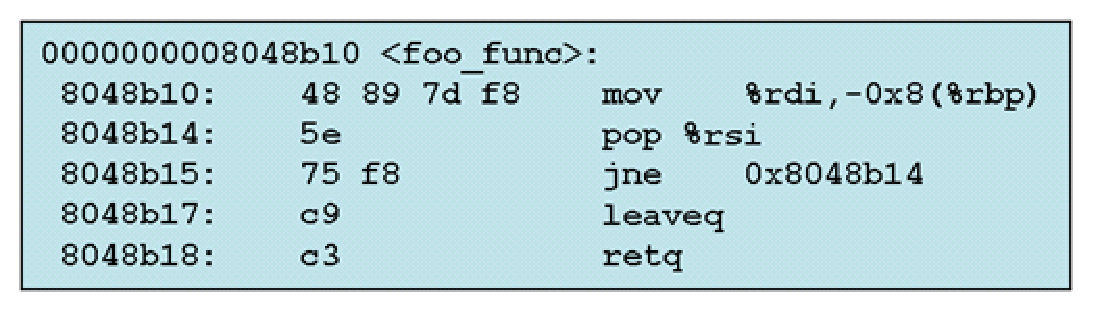
\includegraphics[scale=0.36]{funcp1.eps}
}
\hspace{5mm}
\subfigure[The application function after it has been relocated and the old function entry has been linked to it.]{
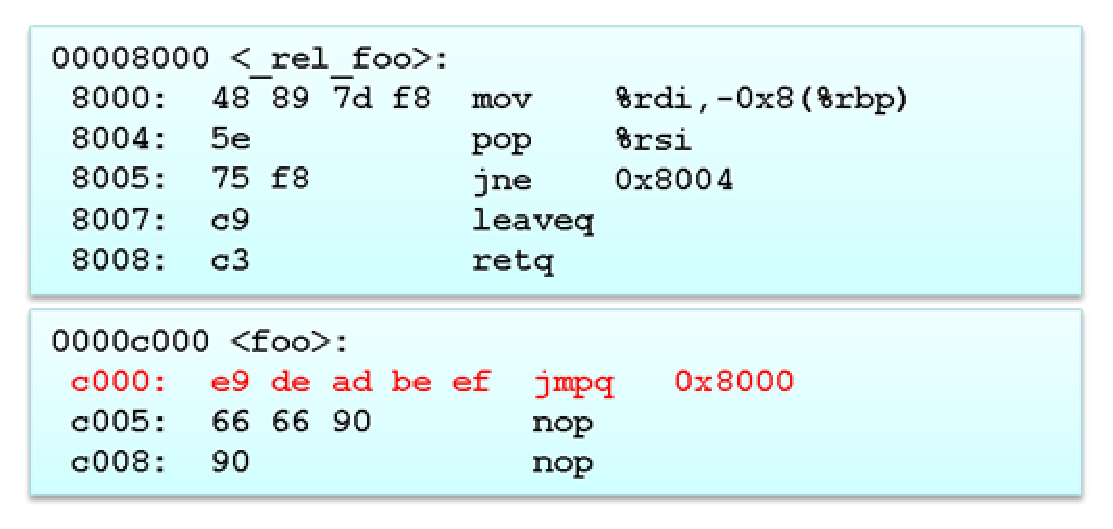
\includegraphics[scale=0.36]{funcp2.eps}
}
\hspace{5mm}
\subfigure[The application function after the branch has been converted to use a 32-bit offset.]{
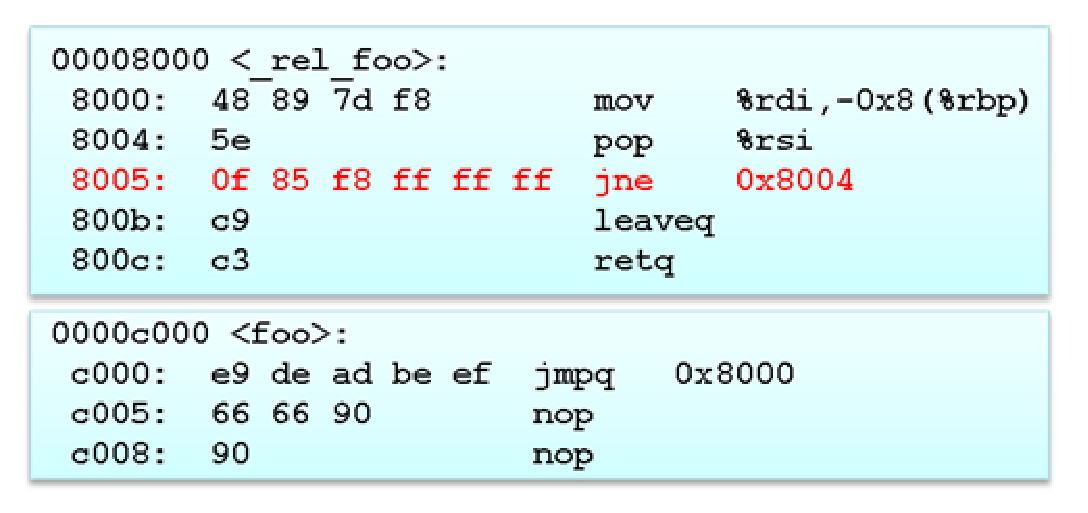
\includegraphics[scale=0.36]{funcp3.eps}
}
\hspace{5mm}
\subfigure[The application function after it has been padded with nop instructions so that each basic block
is large enough to hold a 5 byte jump instruction.]{
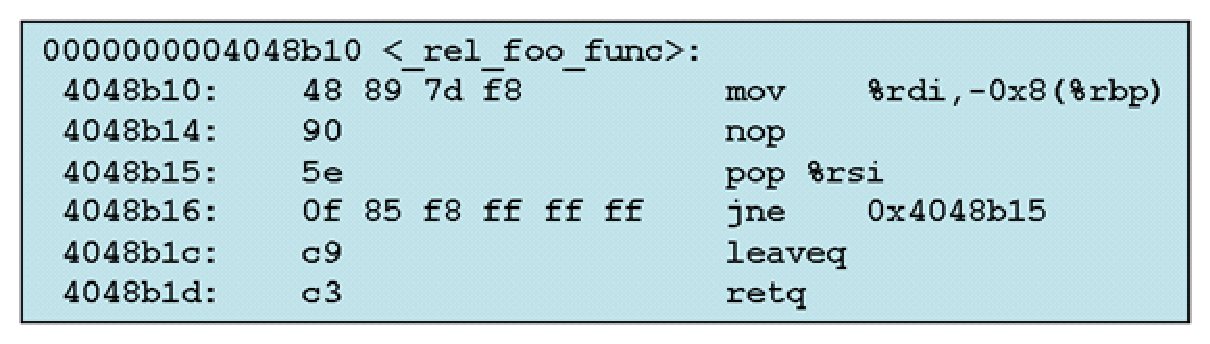
\includegraphics[scale=0.36]{funcp4.eps}
}
\hspace{5mm}
\subfigure[The application function after a single basic block (Basic Block 1) has been instrumented.]{
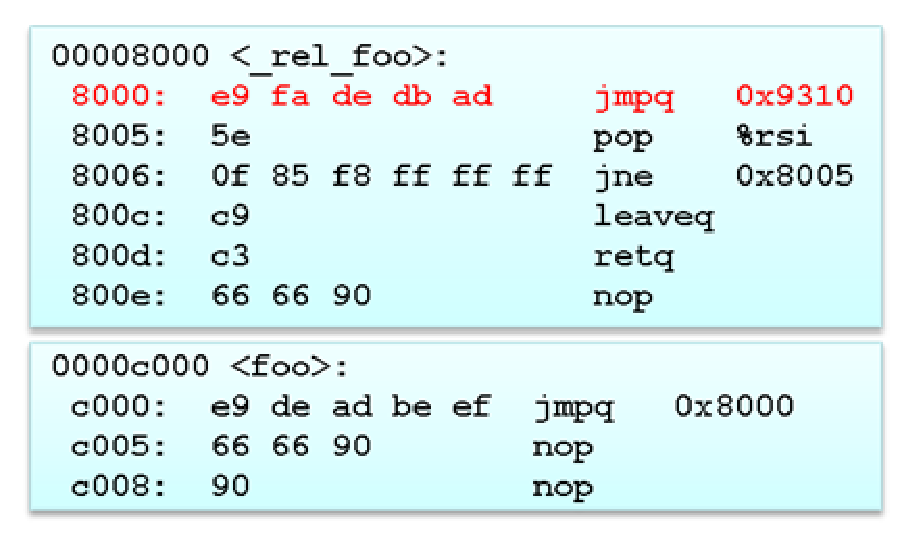
\includegraphics[scale=0.36]{funcp5.eps}
}
\end{figure}


Figure \ref{fig:Relocation}(a) shows a function body prior to any
relocation/instrumentation activities. \textit{Function Displacement + Entry
Point Linking}, shown in Figure \ref{fig:Relocation}(b), relocates the contents
of the entire function to an area of the text section allocated for use by the
instrumentation text. This is done because functions are often packed tightly
together. As a result it is generally not possible to leave a function's entry
point undisturbed and expand its size in a straightforward way without
disturbing the entry point of another nearby function. The original entry point
of the function is then linked to the new location by inserting
an unconditional branch at the original function entry to transfer control to
the displaced function entry. Linking is done in this fashion because most
references to the entry point of a function are in the form of function calls,
which routinely are indirect references (i.e. their value is computed or looked
up at runtime) and are difficult to resolve prior to runtime. \textit{Branch
Conversion}, shown in Figure \ref{fig:Relocation}(c), converts each short branch
in the relocated function to the equivalent 5 byte branch instruction. Since the
code is being reorganized in the next step, which may strain the limits of
smaller 8-bit or 16-bit offsets, all branches are converted to use 32-bit
offsets so that the targets of each branch will still be reachable without the
need to make further changes to the code. Note that there may be some
opportunity here to reduce space by using the smallest branch offset size that
accommodates the branch, but currently a single unified technique is used
to simplify the implementation. Our experiments in Section
\ref{sec:Results} also indicate that the opportunities for improving efficiency
for this technique are minimal. \textit{Instruction Padding}, seen in Figure
\ref{fig:Relocation}(d), pads each instrumentation point, in this case each
basic block, with \begin{it}nop\end{it} instructions so that a 5 byte branch can
be accommodated. \textit{Instrumentation} replaces the instructions at each
instrumentation point with a jump that transfers control to the instrumentation
code, which is shown in Figure \ref{fig:Relocation}(e).

There are several ways that whole function relocation may adversely affect the
performance of the instrumented executable apart from of the overhead that
will be imposed by the instrumentation code. Each function call now
has an extra control interruption associated with it since control must be
passed first to the original function entry point and then to the relocated
function entry point. In addition it is possible that using 32-bit offsets for
every branch rather than some smaller number of bits has an overhead associated
with it. Since the code is being reorganized and expanded, some positive
alignment and size optimizations that the compiler might have made on the
instructions in the function might be destroyed. Finally our technique
introduces extra instructions to be executed in the form of nops.

To quantify the impact of function relocation and the other organizational
changes on application performance, we generated executables in which functions
are relocated, branches are converted to use 32-bit offsets, instruction padding
is applied, yet no instrumentation is introduced. These executables can be used
to measure the overhead of the transformations applied to the executable in
order to prepare it for instrumentation independent of any overhead imposed by
the instrumentation itself. The overhead on a set of ten of the SPECINT 2000
benchmarks never exceeds 6.5\%, with an average overhead of just 1.6\%. Thus the
basic overhead incurred by code relocation and transformation in PEBIL to
accommodate all instrumentation points is well within reason and does not
represent a significant hurdle for efficiency of the instrumented code.

\subsection{Efficient Instrumentation Snippets}

With many instrumentation toolkits, the tasks performed by the instrumentation
tool are accomplished by allowing the user to transfer control from
instrumentation points in the application to instrumentation functions provided
by the user, typically via a shared library or some object code. Since these
instrumentation functions are delivered via a shared library or other object
code, the instrumentation tool developer has the advantage of being able to use
a software development toolchain to write the code in a language that
compiles to the underlying object code. However, the instrumentation function as
a functional mechanism is heavyweight due to the overhead of performing a
function invocation including saving the complete machine state for all
possibles cases that occur in the function. In cases where efficiency is
important, it can be more desirable to insert small sequences of assembly code
to perform a task and only save the small subset of machine state that will be
affected rather than relying entirely on instrumentation functions and the more
costly state preservation that comes with their use.

Most of this state preservation is in the form of register saving and restoring,
but some of it comes in the form of protecting the application call stack from
the instrumentation function. The call stack requires protection from the
instrumentation code during execution because compilers will often optimize leaf
functions in the application by not explicitly creating a stack frame for the
local function data to operate in. This optimization is safe for the application
because during its normal execution a leaf function will never call another
function and thus its wayward stack contents can never be destroyed. In the case
of an instrumented application that calls an instrumentation function from a
leaf, this guarantee no longer holds. Thus, the area above the stack needs to be
protected when an instrumentation function is called from a leaf function.
During the disassembly of a function, PEBIL notes whether it is a leaf function
(i.e. whether it contains any call instructions). Later, during instrumentation,
it automatically protects the stack contents from any instrumentation function
calls made from that function by incrementing the stack pointer by a fixed
amount\footnote{Currently this amount is set to 4 kilobytes, which is large
enough to accommodate the stack usage of all of the leaf functions we have
encountered so far}, which has the effect of giving the leaf function a large
fixed-size stack frame while the instrumentation function is active.

A good example of the efficiency of using instrumentation snippets rather than
instrumentation functions is an instrumentation point at which the desired
outcome for the instrumentation tool is to increment a counter that resides in
memory. In order to accomplish this task with an instrumentation snippet,
control is transferred to the instrumentation point's trampoline which will save
the platform's flags register, update the counter in memory, restore the flags
register, then transfer control back to the application. If instead one used an
instrumentation function, prior to performing the task, the trampoline must save
the flags register, any registers used by the function, and possibly perform
stack protection. It also requires at least 2 more control transfers in order to
enter and exit the instrumentation function. Furthermore these control flow
transfers generally use the call/return paradigm, which in addition to changing
the application's program counter will also store and retrieve information about
the function call site onto the stack, making the use of a snippet a more
efficient choice.

In addition, the use of the instrumentation function is also likely to pollute
the instruction cache more than using a compact instrumentation snippet. For an
instrumentation snippet the application code must contend with the trampoline
code only, whereas using an instrumentation function puts the function code in
contention with the application and the trampoline. Hence, instrumentation
functions tend to be more heavyweight than instrumentation snippets and using
snippets rather than functions whenever possible allows us to gather
\textit{asynchronous} program information more efficiently. Intuitively,
asynchronous information can be thought of as any information that could be
dumped to disk and processed offline. Gao et. al. \cite{gao2005aliter}
demonstrate that using lightweight instrumentation snippets to buffer
information which is later processed by more heavyweight instrumentation
functions in batches is an efficient yet entirely lossless way for
instrumentation tools to process asynchronous program information. The
availability of instrumentation snippets gives tool developers the flexibility
to choose either snippets or functions depending on their performance goals and
software engineering needs.
